% !TEX engine = lualatex
\documentclass[aspectratio=169,handout,usepdftitle=false]{fireshonks}

%%%%%%%%%%%%%%%%%%%%%
% PAQUETES
%%%%%%%%%%%%%%%%%%%%%

\setdefaultlanguage{english}
\setotherlanguage[variant=austrian]{german}
\usepackage{tikz}
\usetikzlibrary{arrows.meta, matrix, shapes.geometric, overlay-beamer-styles}
\usepackage[german]{datetime2}
\usepackage{subcaption}
\usepackage{import}
\usepackage{siunitx}
\usepackage{fontawesome5}
\usepackage{emoji}
\sisetup{mode=text, per-mode=symbol}
\captionsetup{font+=scriptsize,justification=centering}
\usepackage{tabularray}
\UseTblrLibrary{booktabs}
\usepackage{qrcode}

%%%%%%%%%%%%%%%%%%%%%
% TEMPLATE
%%%%%%%%%%%%%%%%%%%%%
% Title graphics: BG + logo of the conference
\titlegraphic{
  \begin{tikzpicture}[remember picture, overlay]
    \mode<beamer>{\scoped[on background layer]\node [centered,opacity=0.4] at (current page.center) {
\includegraphics[width=\pagewidth,height=\pageheight,keepaspectratio]{frontmatter/cropped-Try_This_At_Home-1920x1080-1.png}};}
    \scoped[on background layer]\node [below left] at (current page.north east) {
\includegraphics[height=4em,keepaspectratio]{frontmatter/annie-shenanigans}};
    % Background: FireShonks  \\
    \scoped[on background layer]\node [above right,align=left,font=\tiny\itshape] at (current page.south west) {
      Seal: \href{https://lethalbit.net}{Aki Van Ness}, CC-BY-SA-4.0
    };
  \end{tikzpicture}
}

%%%%%%%%%%%%%%%%%%
% METADATA
%%%%%%%%%%%%%%%%%%

\title{The Unsung Heroes of Imaging}
\author{amyspark}
\date{\DTMdate{2023-12-27}}

\addbibresource{bibliography.bib}

\begin{document}
\maketitle

\begin{frame}{About me}
    \begin{itemize}[<*>]
        \item Upstreamer \& Compiler Breaker at Centricular
              \begin{itemize}[<*>]
                  \item Fine purveyors of Free and Open Source Software consulting
                  \item Maintainers of the GStreamer multimedia framework
              \end{itemize}
        \item Colour spaces, SIMD, build systems... curses are my specialty \emoji{woman-mage}
        \item Occasional contributor to a lot of projects
    \end{itemize}
\end{frame}
\begin{frame}{Motivation}
    \begin{itemize}
        \item Most of you may understand terms like \enquote{JPG picture}, \enquote{PNG}, even \enquote{TIFF}...
        \item Watching TV? You may have heard about \enquote{PAL}, \enquote{NTSC}, \enquote{SECAM}
        \item How do we store and broadcast colour images?
    \end{itemize}
\end{frame}

\begin{frame}{Motivation}
    \begin{itemize}
        \item Why is a JPEG picture so small compared to PNG, TIFF, RAW...?
        \item How can we watch \emoji{cat} videos on phones?
        \item How were we able to watch colour TV before the PC era?
        \item \emoji{woman-mage} there's a \emph{luma-chroma colour space} involved to compress them!
        \item Lots of background to cover, includes HDR too!
    \end{itemize}
\end{frame}
\begin{frame}{Scope}
    \tableofcontents
\end{frame}
\section{Introduction}
\begin{frame}{How are colours specified?}
    Colours are specified as coordinates in a \emph{colour space}.
    \begin{itemize}[<+(1)->]
        \item $n$-dimensional geometrical model
        \item light stimuli (colours) $\leftrightarrow$ vector coordinates
        \item If you've taken a picture, or browsed the web, you've run across them
              \begin{itemize}
                  \item the sRGB colour space powers most consumer content nowadays
              \end{itemize}
    \end{itemize}
\end{frame}
\begin{frame}{Colour spaces as a mathematical construct}
    \begin{itemize}
        \item Coordinate system
        \item A subspace within that system
        \item A mapping function from a \emph{supported} colour to a single point inside the subspace
        \item The set of supported colours is the colour space's \emph{gamut}
    \end{itemize}
\end{frame}
\begin{frame}{Formal definition of a colour space}
    \begin{columns}<.->
        \begin{column}<.->{.7\textwidth}
            \begin{itemize}
                \item Two sets of components:
                      \begin{enumerate}
                          \item Three independent, reference stimuli: \emph{primaries}
                          \item Colour of the light source: white point or \emph{illuminant}
                      \end{enumerate}
                \item These components are represented by their \emph{chromaticity} coordinates
                \item Plotting them in \emph{chromaticity diagrams} reveals the space's gamut
            \end{itemize}
        \end{column}
        \begin{column}<.->{.3\textwidth}
            \begin{figure}
                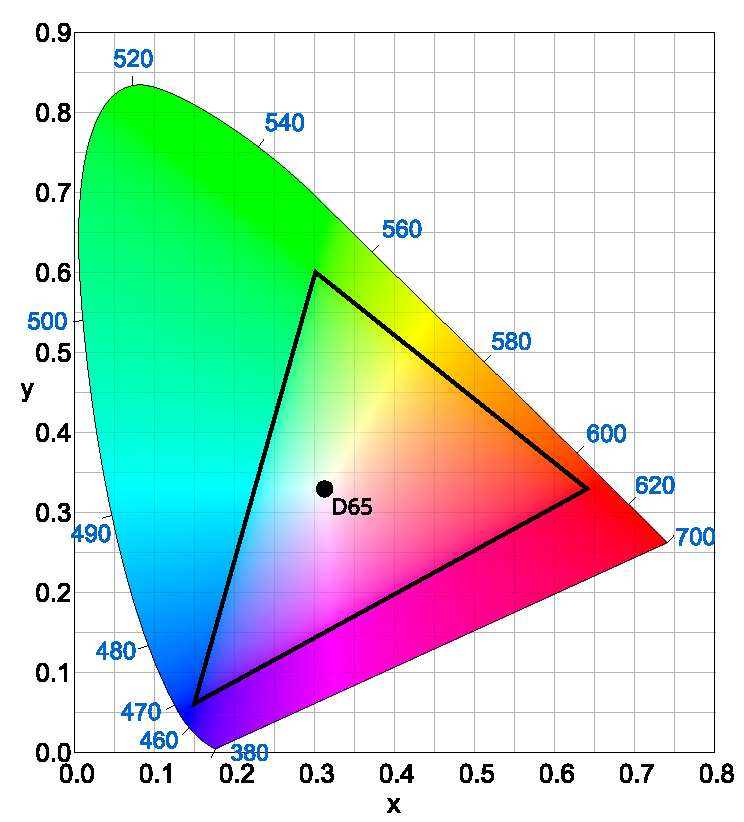
\includegraphics[width=\columnwidth,keepaspectratio]{figures/bt709.pdf}
                \caption*{The colour space of ITU-R BT.709. Source: \href{https://commons.wikimedia.org/wiki/File:CIExy1931_Rec_709.svg}{GrandDrake}, \href{http://creativecommons.org/licenses/by-sa/3.0/}{CC BY-SA 3.0}, via Wikimedia Commons}
            \end{figure}
        \end{column}
    \end{columns}
\end{frame}
\begin{frame}{How are colours stored and transmitted?}
    It's essential to understand at which \enquote{stage} we're at:
    \begin{enumerate}
        \item Colour \emph{model}
        \item Colour \emph{space}
        \item Colour \emph{encoding}
    \end{enumerate}
\end{frame}
\begin{frame}{Example: the sRGB colour space}
    \emph{sRGB} ("standard RGB") powers most consumer content nowadays
    \begin{itemize}
        \item Type: additive
              \begin{itemize}
                  \item works by \emph{adding light} to represent colours
                  \item there are \emph{subtractive} colour spaces too, not covered here
              \end{itemize}
        \item Model: RGB
              \begin{itemize}
                  \item Three coordinates: $(r, g, b)$ for red, green, and blue
              \end{itemize}
        \item Definition: \href{https://www.evs.ee/en/evs-en-61966-2-1-2002}{ISO IEC 61966-2-1}
        \item Encoding: most standards provide conversion formulae for the intended bit depth
              \begin{itemize}
                  \item this one is designed for \emph{8-bit unsigned integer}
              \end{itemize}
    \end{itemize}
\end{frame}
\begin{frame}{Colour management}
    \begin{itemize}
        \item In the analog era, there was a single colour space
              \begin{itemize}
                  \item Standardized in Recommendations from the International Telecommunications Union
                  \item eg. ITU.R BT-709 \parencite{BT709} for digital SD TV content
                  \item there were variations in broadcasting standards -- we'll cover these later
              \end{itemize}
        \item In the digital era, we need \emph{colour management systems}
    \end{itemize}
\end{frame}
\begin{frame}{Colour management}
    \begin{itemize}
        \item Modern colour management systems follow the International Colour Consortium's framework \autocite{allen}
        \item \emph{Open-loop} colour management
        \item Calculations are done in a \emph{profile connection space} (PCS)
        \begin{itemize}
            \item Intermediate, device-independent colour space
            \item Primaries and illuminant are defined in this colour space
        \end{itemize}
        \item Conversions to/from each device $\equiv$ \emph{transformation} from/to the PCS
              \begin{itemize}
                  \item (note the inverted directions)
              \end{itemize}
    \end{itemize}
\end{frame}
\begin{frame}{Open-loop colour management}
    \begin{figure}
        \begin{tikzpicture}[
                node distance=3em and 5em,
                device/.style={align=center, font=\Large},
                pcs/.style={circle, text width=3em, align=center, draw},
                transform/.style={->,shorten >=1pt,>=Latex,semithick}
            ]
            \node (i1) [device] {\emoji{camera}};
            \node (i2) [device, below=of i1] {\emoji{video-camera}};
            \node (i3) [device, below=of i2] {\emoji{movie-camera}};
            \node (pcs) [pcs, right=of i2] {PCS};
            \node (d1) [device, above=of pcs] {\emoji{desktop-computer}};
            \node (d2) [device, below=of pcs] {\emoji{mobile-phone}};
            \node (o1) [device, above right=of pcs] {\emoji{printer}};
            \node (o2) [device, below right=of pcs] {\emoji{printer}};

            \draw[transform] (i1) -- (pcs) node [midway, visible on=<2->] {\emoji{arrows-counterclockwise}};
            \draw[transform] (i2) -- (pcs) node [midway, visible on=<2->] {\emoji{arrows-counterclockwise}};
            \draw[transform] (i3) -- (pcs) node [midway, visible on=<2->] {\emoji{arrows-counterclockwise}};
            \draw[transform] (i1) -- (pcs) node [midway, visible on=<2->] {\emoji{arrows-counterclockwise}};
            \draw[transform] (pcs) -- (d1) node [midway, visible on=<2->] {\emoji{arrows-counterclockwise}};
            \draw[transform] (pcs) -- (d2) node [midway, visible on=<2->] {\emoji{arrows-counterclockwise}};
            \draw[transform] (pcs) -- (o1) node [midway, visible on=<2->] {\emoji{arrows-counterclockwise}};
            \draw[transform] (pcs) -- (o2) node [midway, visible on=<2->] {\emoji{arrows-counterclockwise}};
        \end{tikzpicture}

        \caption*{Adapted from \textcite[viii]{icc}}
    \end{figure}
\end{frame}
\begin{frame}{The ICC colour management architecture}
    Four key components:
    \begin{enumerate}[<+(1)->]
        \item The PCS
        \item The \emph{colour management module}
              \begin{itemize}
                  \item A software library that performs all the colour conversions
                  \item Usually embedded on your OS, there are also vendor offerings available
              \end{itemize}
        \item The device profiles
              \begin{itemize}
                  \item Contain the data to transform between PCS and the device's colour space
                  \item \emoji{woman-mage} our spaces are here
              \end{itemize}
        \item Rendering \emph{intents}
              \begin{itemize}
                  \item Exact matches between spaces may not be possible: \emph{out-of-gamut} colours
                  \item The CMS needs to \emph{predictably} account for this
              \end{itemize}
    \end{enumerate}
\end{frame}
\begin{frame}{The ICC colour management architecture}
    \begin{center}
        Interested? Watch my talk at DiVOC!

        \qrcode[hyperlink,height=4\baselineskip]{https://media.ccc.de/v/divoc_bb3-48292-the-last-frontier-on-icc-profiles}

        \url{https://media.ccc.de/v/divoc_bb3-48292-the-last-frontier-on-icc-profiles}
    \end{center}
\end{frame}
\section{What are these spaces for?}
\begin{frame}{}

    

\end{frame}

\begin{frame}{What is YCbCr?}
    \begin{center}
        Device independent colour space encoding
    \end{center}

    \begin{itemize}[<+(1)->]
        \item \emph{Device-independent:} its specification is fixed and does not depend on a particular device
        \item \emph{Colour space:} it is a mathematical transformation of RGB
        \item \emph{Encoding:} it specifies
              \begin{itemize}
                  \item the digital encoding method (8 or 10-bit unsigned integer, floating point)
                  \item the encoding range (it depends for each of the options)
              \end{itemize}
    \end{itemize}
\end{frame}
\section{Examples}
\begin{frame}{Reasoning}
    \begin{center}
        Digital encoding of colour signals for TV
    \end{center}

    \uncover<+(1)->{What does it need to cover? \autocite{tooms}}
    \begin{enumerate}[<+(1)->]
        % Tooms 14.2.1
        \item Retaining colour balance
              \begin{itemize}
                  \item colour drifts between different cameras? \emoji{pleading-face}
              \end{itemize}
        \item Compatibility with monochrome (grayscale) systems
              \begin{itemize}
                  \item split the signal into \emph{luminance} and \emph{chromaticity} components
              \end{itemize}
        \item Efficiency of the colour signal(s)
              \begin{itemize}
                  \item e.g. a single 1080p frame, 8-bit RGB uncompressed, is \SI{170}{\mega\byte}
              \end{itemize}
    \end{enumerate}
\end{frame}
\begin{frame}{YIQ}
    \begin{columns}<.->
        \begin{column}<.->{.7\textwidth}
            \begin{itemize}
                \item $(R, G, B)$ pixel $\rightarrow$ $(Y, Cb, Cr)$ signal values
                \item $Y$ is the \emph{luminance} signal
                      \begin{itemize}
                          \item Intuitively, our eyes are most sensitive to $G$
                          \item $G$ is a major contributor to the luminance value
                          \item $R$ and $B$ have smaller contributions
                      \end{itemize}
                \item $Cb$ and $Cr$ together form the \emph{chrominance} signal
                      \begin{itemize}
                          \item complementary \emph{colour difference} signals
                          \item $Cb$ blue - luma, $Cr$ red - luma
                      \end{itemize}
                \item Standardized by the ITU in two Recommendations
            \end{itemize}
        \end{column}
        \begin{column}<1->{.3\textwidth}
            \begin{figure}
                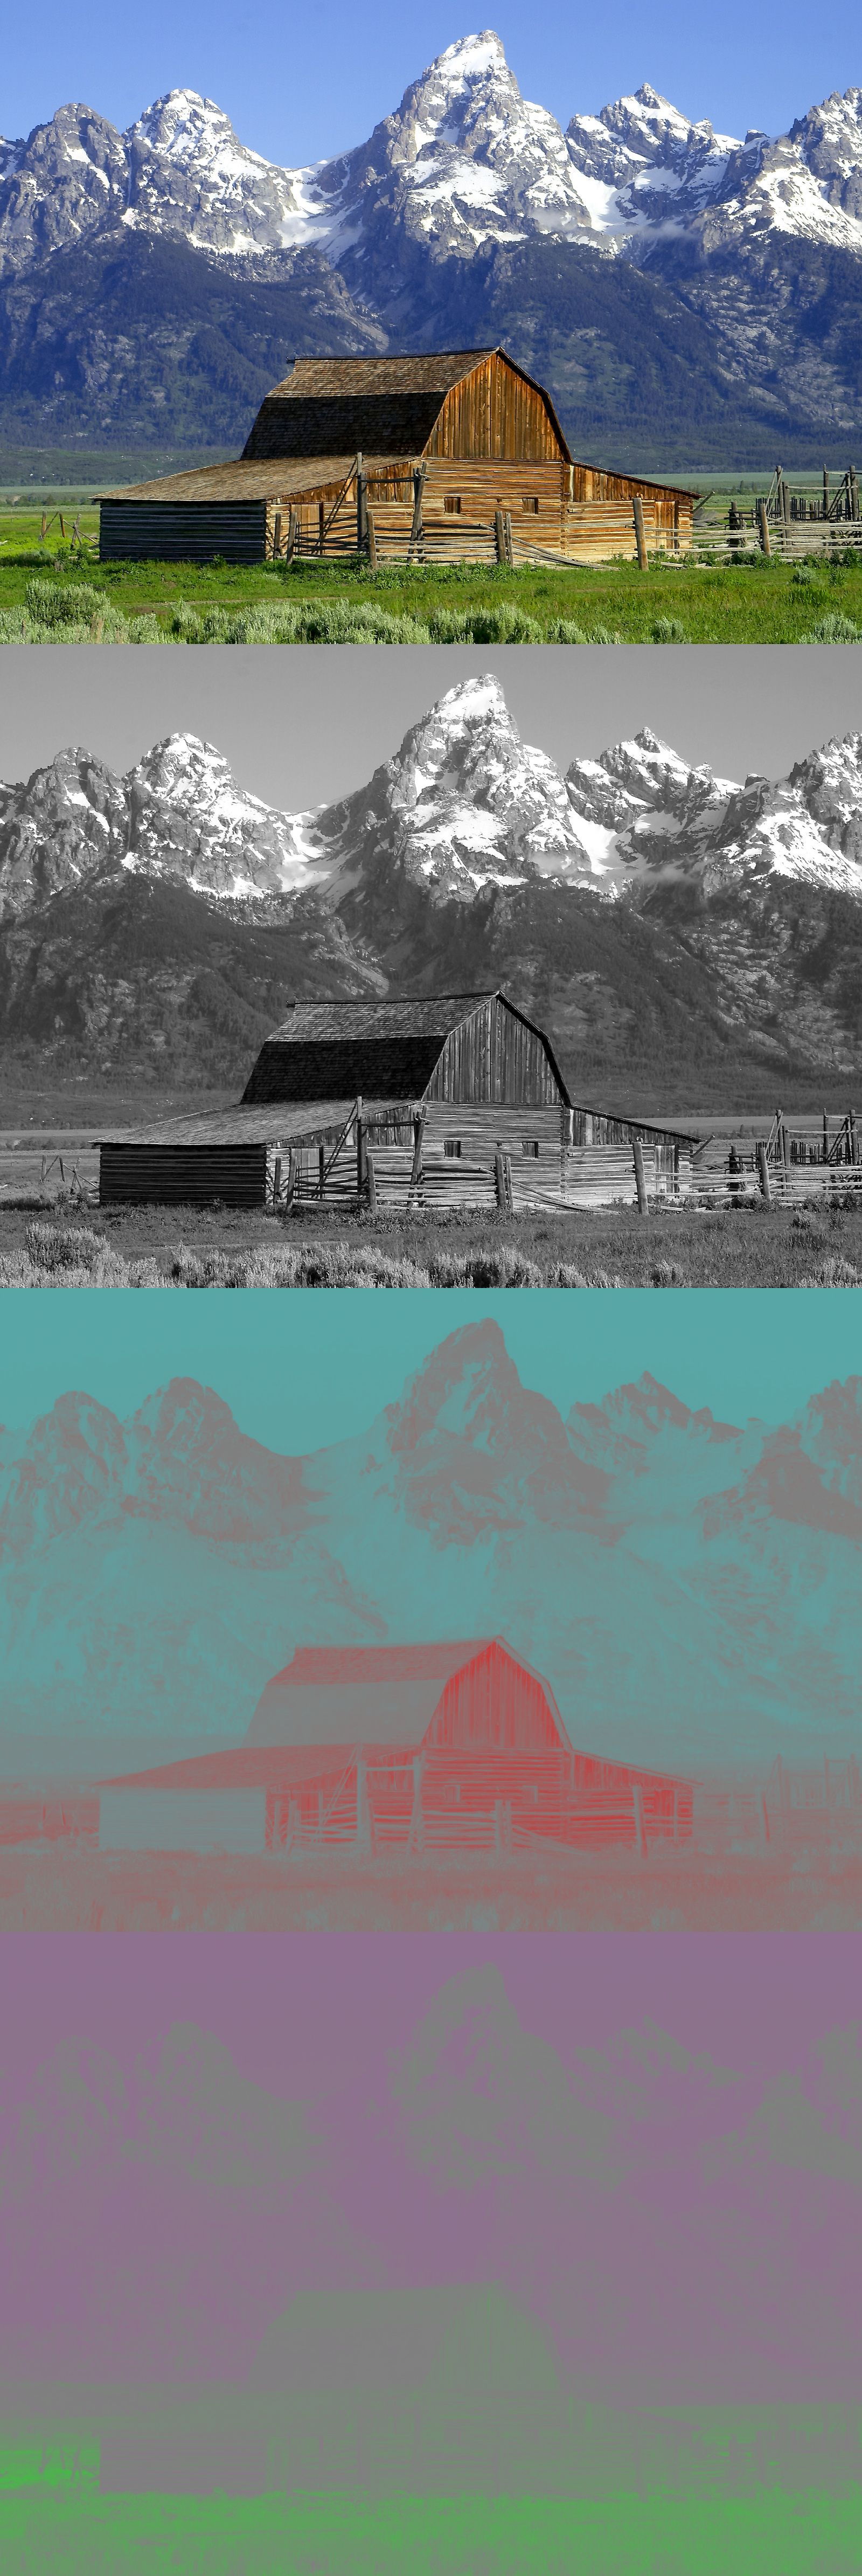
\includegraphics[height=10\baselineskip,keepaspectratio]{figures/YIQ_components.jpg}
                \caption*{Source: \href{https://commons.wikimedia.org/wiki/File:YIQ_components.jpg}{(3ucky(3all}, CC-BY-SA 3.0, via Wikimedia Commons}
            \end{figure}
        \end{column}
    \end{columns}
\end{frame}
\begin{frame}{What does YCbCr do?}
    \begin{columns}<.->
        \begin{column}<.->{.7\textwidth}
            \begin{itemize}
                \item $(R, G, B)$ pixel $\rightarrow$ $(Y, Cb, Cr)$ signal values
                \item $Y$ is the \emph{luminance} signal
                      \begin{itemize}
                          \item Intuitively, our eyes are most sensitive to $G$
                          \item $G$ is a major contributor to the luminance value
                          \item $R$ and $B$ have smaller contributions
                      \end{itemize}
                \item $Cb$ and $Cr$ together form the \emph{chrominance} signal
                      \begin{itemize}
                          \item complementary \emph{colour difference} signals
                          \item $Cb$ blue - luma, $Cr$ red - luma
                      \end{itemize}
                \item Standardized by the ITU in two Recommendations
            \end{itemize}
        \end{column}
        \begin{column}<1->{.3\textwidth}
            \begin{figure}
                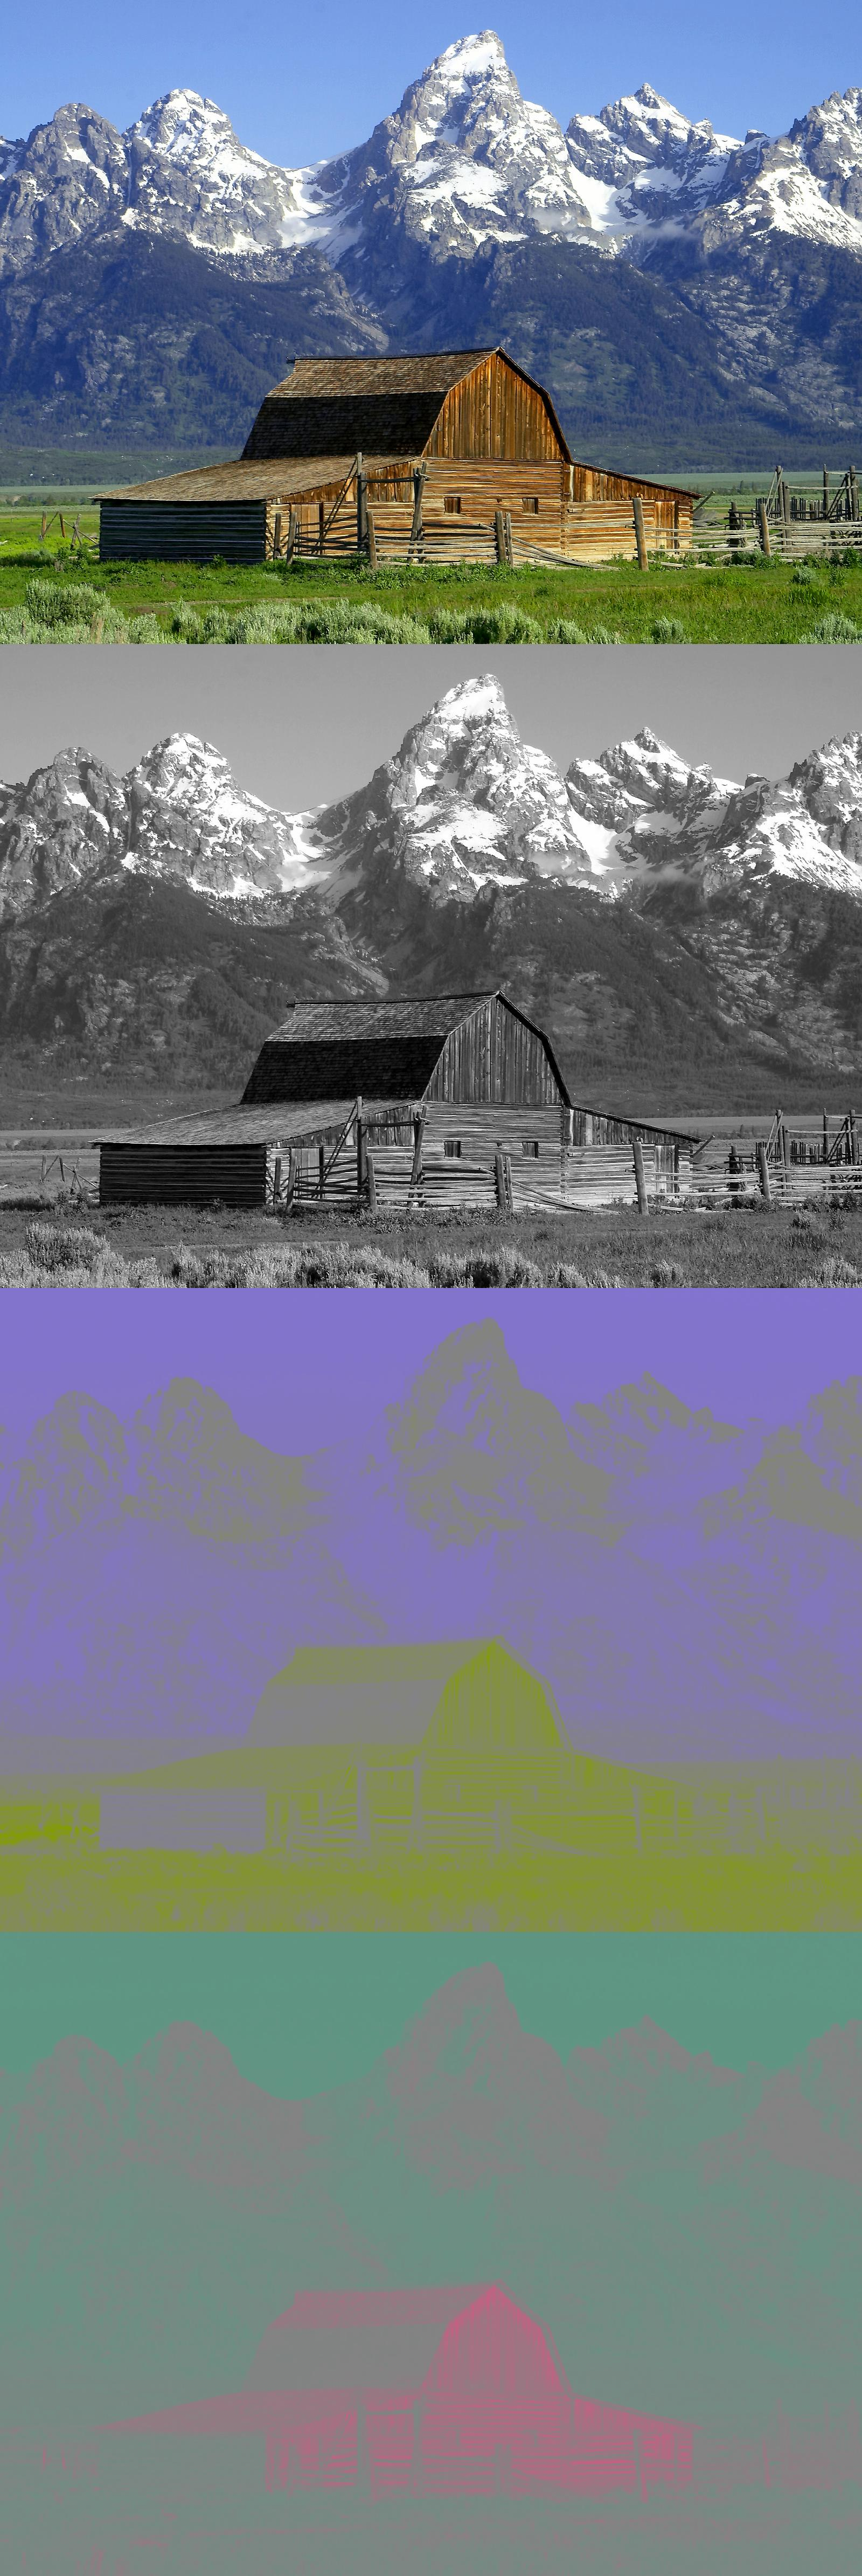
\includegraphics[height=10\baselineskip,keepaspectratio]{figures/Barns_grand_tetons_YCbCr_separation.jpg}
                \caption*{Source: \href{https://commons.wikimedia.org/wiki/File:Barns_grand_tetons_YCbCr_separation.jpg}{Mike1024}, Public domain, via Wikimedia Commons}
            \end{figure}
        \end{column}
    \end{columns}
\end{frame}
\begin{frame}{YCbCr: BT.601-7}
    \begin{itemize}
        \item Last updated in 2011 \autocite{BT601}
        \item Targets standard definition transmissions ($\leq$480p)
        \item Designed for compatibility with legacy receivers
        \item Targets the \emph{D65} white point
    \end{itemize}

    \uncover<+->{
        \begin{align}
            Y' & = 0.299R' + 0.587G' + 0.114B'                                             \\
            Cb & = \frac{0.701}{1.402}R' + \frac{-0.587}{1.402}G' + \frac{-0.114}{1.402}B' \\
            Cr & = \frac{-0.299}{1.772}R' + \frac{-0.587}{1.772}G' + \frac{0.886}{1.772}B'
        \end{align}
    }
\end{frame}
\begin{frame}{YCbCr: BT.709-6 version}
    \begin{itemize}
        \item Last updated in 2015 \autocite{BT709}
        \item Revised version targeting HD and HDR transmissions
        \item Drops legacy compatibility in exchange for accurate eye luminance response
        \item Targets the \emph{D65} white point
    \end{itemize}

    \uncover<+->{
        \begin{align}
            Y' & = 0.2126R' + 0.7152G' + 0.0722B'                                                \\
            Cb & = \frac{-0.2126}{1.8556}R' + \frac{-0.7152}{1.8556}G' + \frac{0.9278}{1.8556}B' \\
            Cr & = \frac{0.7874}{1.5748}R' + \frac{-0.7152}{1.5748}G' + \frac{-0.0722}{1.5748}B'
        \end{align}
    }
\end{frame}
\begin{frame}{YCbCr: range}
    \begin{itemize}
        \item Intended for use in analog circuitry
              \begin{itemize}
                  \item e.g. 8-bit unsigned integer: $Y' \in [16, 235]$; $Cb, Cr \in [16, 240]$
                  \item the extra room is to allow for the carrier signal to under/overshoot
              \end{itemize}
        \item Both matrices as well as the ICC standard expect data in floating point
        \item \emoji{woman-raising-hand}: what is the range?
        \item \emoji{woman-mage}: only BT.601 explains it (\S2.5.2)
        \item $Y' \in [0, 1]$; $Cb, Cr \in [-0.5, 0.5]$
    \end{itemize}
\end{frame}
\begin{frame}{YCbCr: gamma correction}
    \begin{itemize}
        \item YCbCr takes/returns a gamma-corrected RGB signal
              \begin{itemize}
                  \item the $'$ in $R'$ earlier denotes that correction
              \end{itemize}
        \item Formally called \emph{opto-electronic transfer function} (OETF)
        \item Accounts for the non-linearity on the image sensor/display device
        \item BT.601 and BT.709 specify the same relationship between luminance $L$ and electrical signal $E$: \begin{equation}
                  E = \begin{cases}
                      (1.099L^{0.045} - 0.099) & 0.018 < L \leq 1.00 \\
                      4.500L                   & 0 \leq L \leq 0.018
                  \end{cases}
              \end{equation}
    \end{itemize}
\end{frame}
\begin{frame}{CRT-style gamma correction}
    \begin{itemize}
        \item There is little info on YCbCr's actual usage so let's consider an alternative
        \item Old-school CRT television sets follow a \emph{power law}
        \item The relationship between emitted light $L$ and driving voltage $V$:
              \begin{equation}
                  L = V^{\gamma}
              \end{equation}
        \item $\gamma$ depends on the device
        \item The official recommendation, ITU-R BT.1886 \parencite*{BT1886} defaults to $\gamma = 2.4$
    \end{itemize}
\end{frame}

\begin{frame}{YDbDr}
    \begin{columns}<.->
        \begin{column}<.->{.7\textwidth}
            \begin{itemize}
                \item $(R, G, B)$ pixel $\rightarrow$ $(Y, Cb, Cr)$ signal values
                \item $Y$ is the \emph{luminance} signal
                      \begin{itemize}
                          \item Intuitively, our eyes are most sensitive to $G$
                          \item $G$ is a major contributor to the luminance value
                          \item $R$ and $B$ have smaller contributions
                      \end{itemize}
                \item $Cb$ and $Cr$ together form the \emph{chrominance} signal
                      \begin{itemize}
                          \item complementary \emph{colour difference} signals
                          \item $Cb$ blue - luma, $Cr$ red - luma
                      \end{itemize}
                \item Standardized by the ITU in two Recommendations
            \end{itemize}
        \end{column}
        \begin{column}<1->{.3\textwidth}
            \begin{figure}
                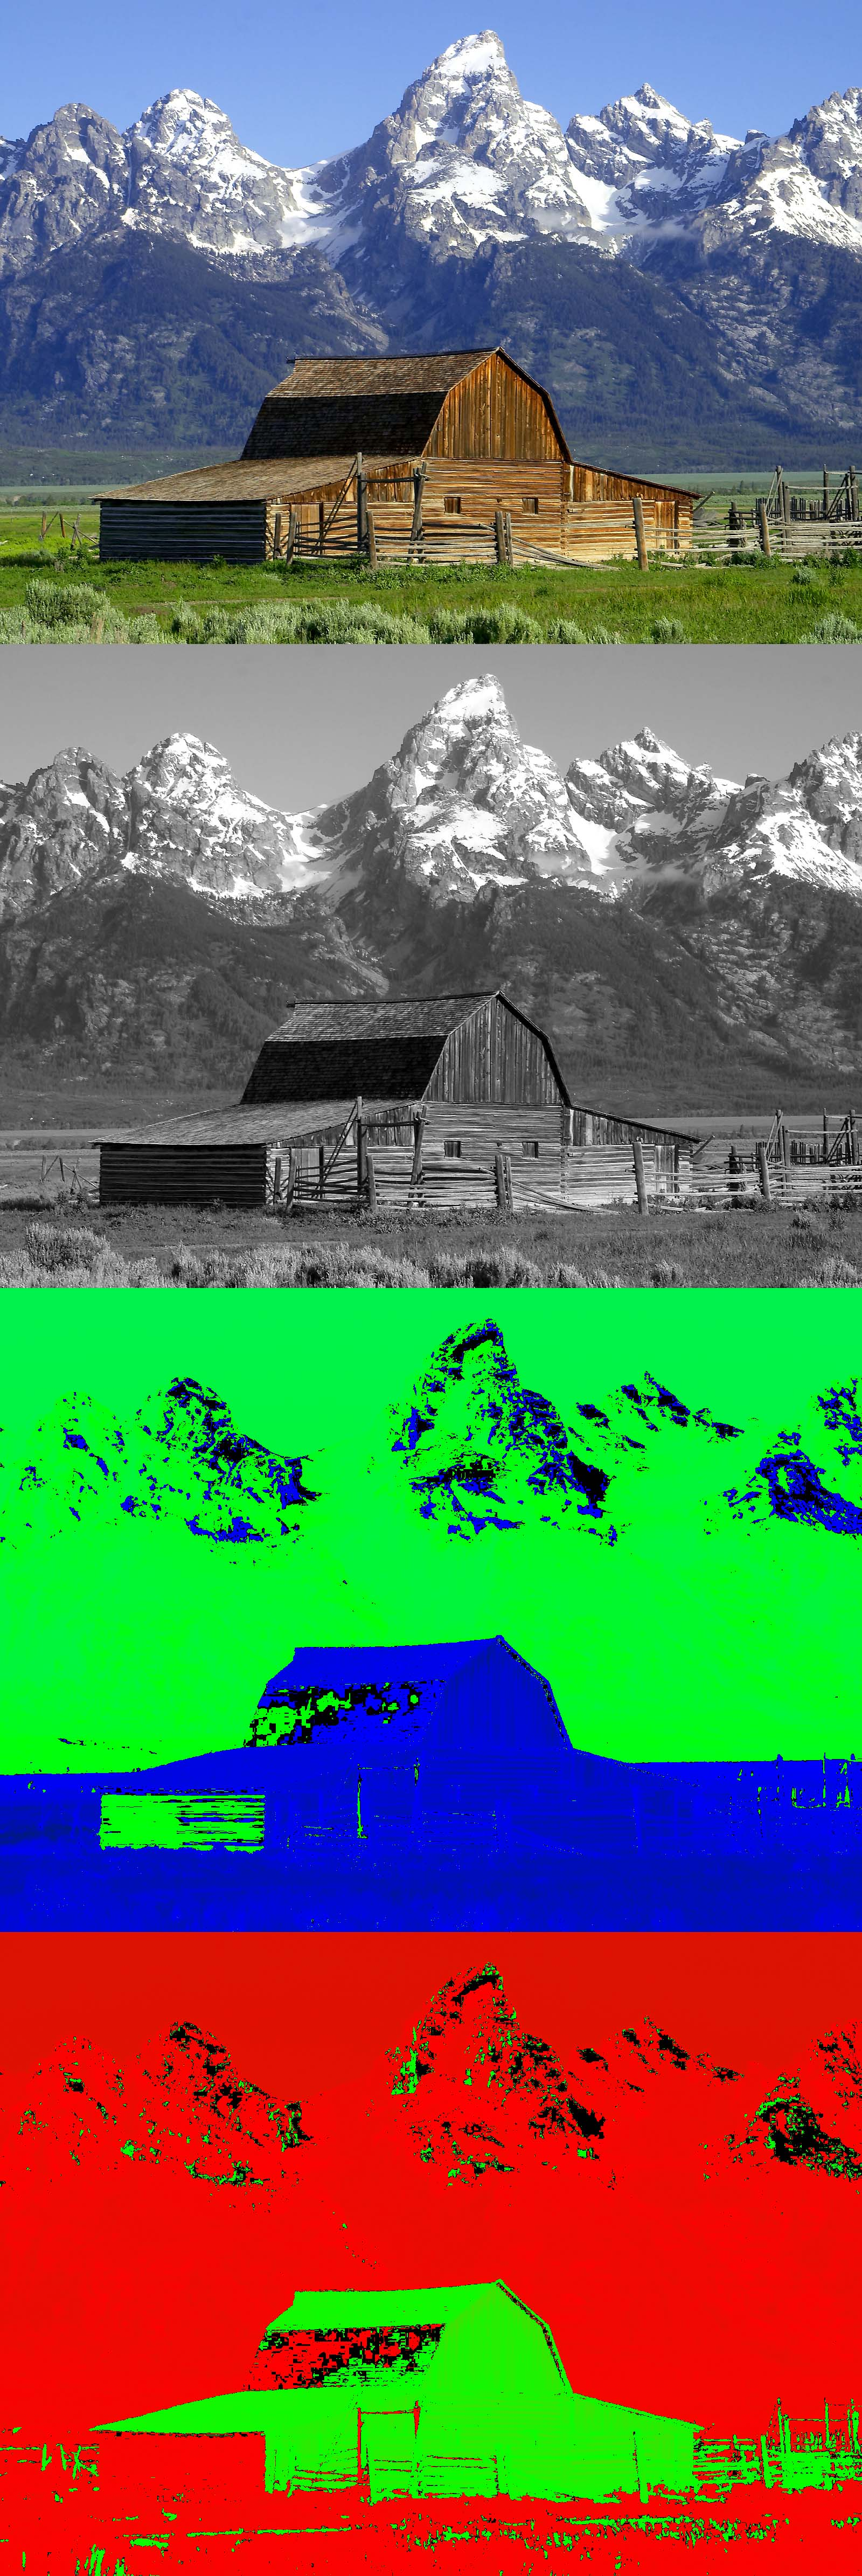
\includegraphics[height=10\baselineskip,keepaspectratio]{figures/YDbDr_components.jpg}
                \caption*{Source: \href{https://commons.wikimedia.org/wiki/File:YDbDr_components.jpg}{(3ucky(3all}, CC-BY-SA 3.0, via Wikimedia Commons}
            \end{figure}
        \end{column}
    \end{columns}
\end{frame}
\begin{frame}{YCgCo}
    \begin{columns}<.->
        \begin{column}<.->{.7\textwidth}
            \begin{itemize}
                \item $(R, G, B)$ pixel $\rightarrow$ $(Y, Cb, Cr)$ signal values
                \item $Y$ is the \emph{luminance} signal
                      \begin{itemize}
                          \item Intuitively, our eyes are most sensitive to $G$
                          \item $G$ is a major contributor to the luminance value
                          \item $R$ and $B$ have smaller contributions
                      \end{itemize}
                \item $Cb$ and $Cr$ together form the \emph{chrominance} signal
                      \begin{itemize}
                          \item complementary \emph{colour difference} signals
                          \item $Cb$ blue - luma, $Cr$ red - luma
                      \end{itemize}
                \item Standardized by the ITU in two Recommendations
            \end{itemize}
        \end{column}
        \begin{column}<1->{.3\textwidth}
            \begin{figure}
                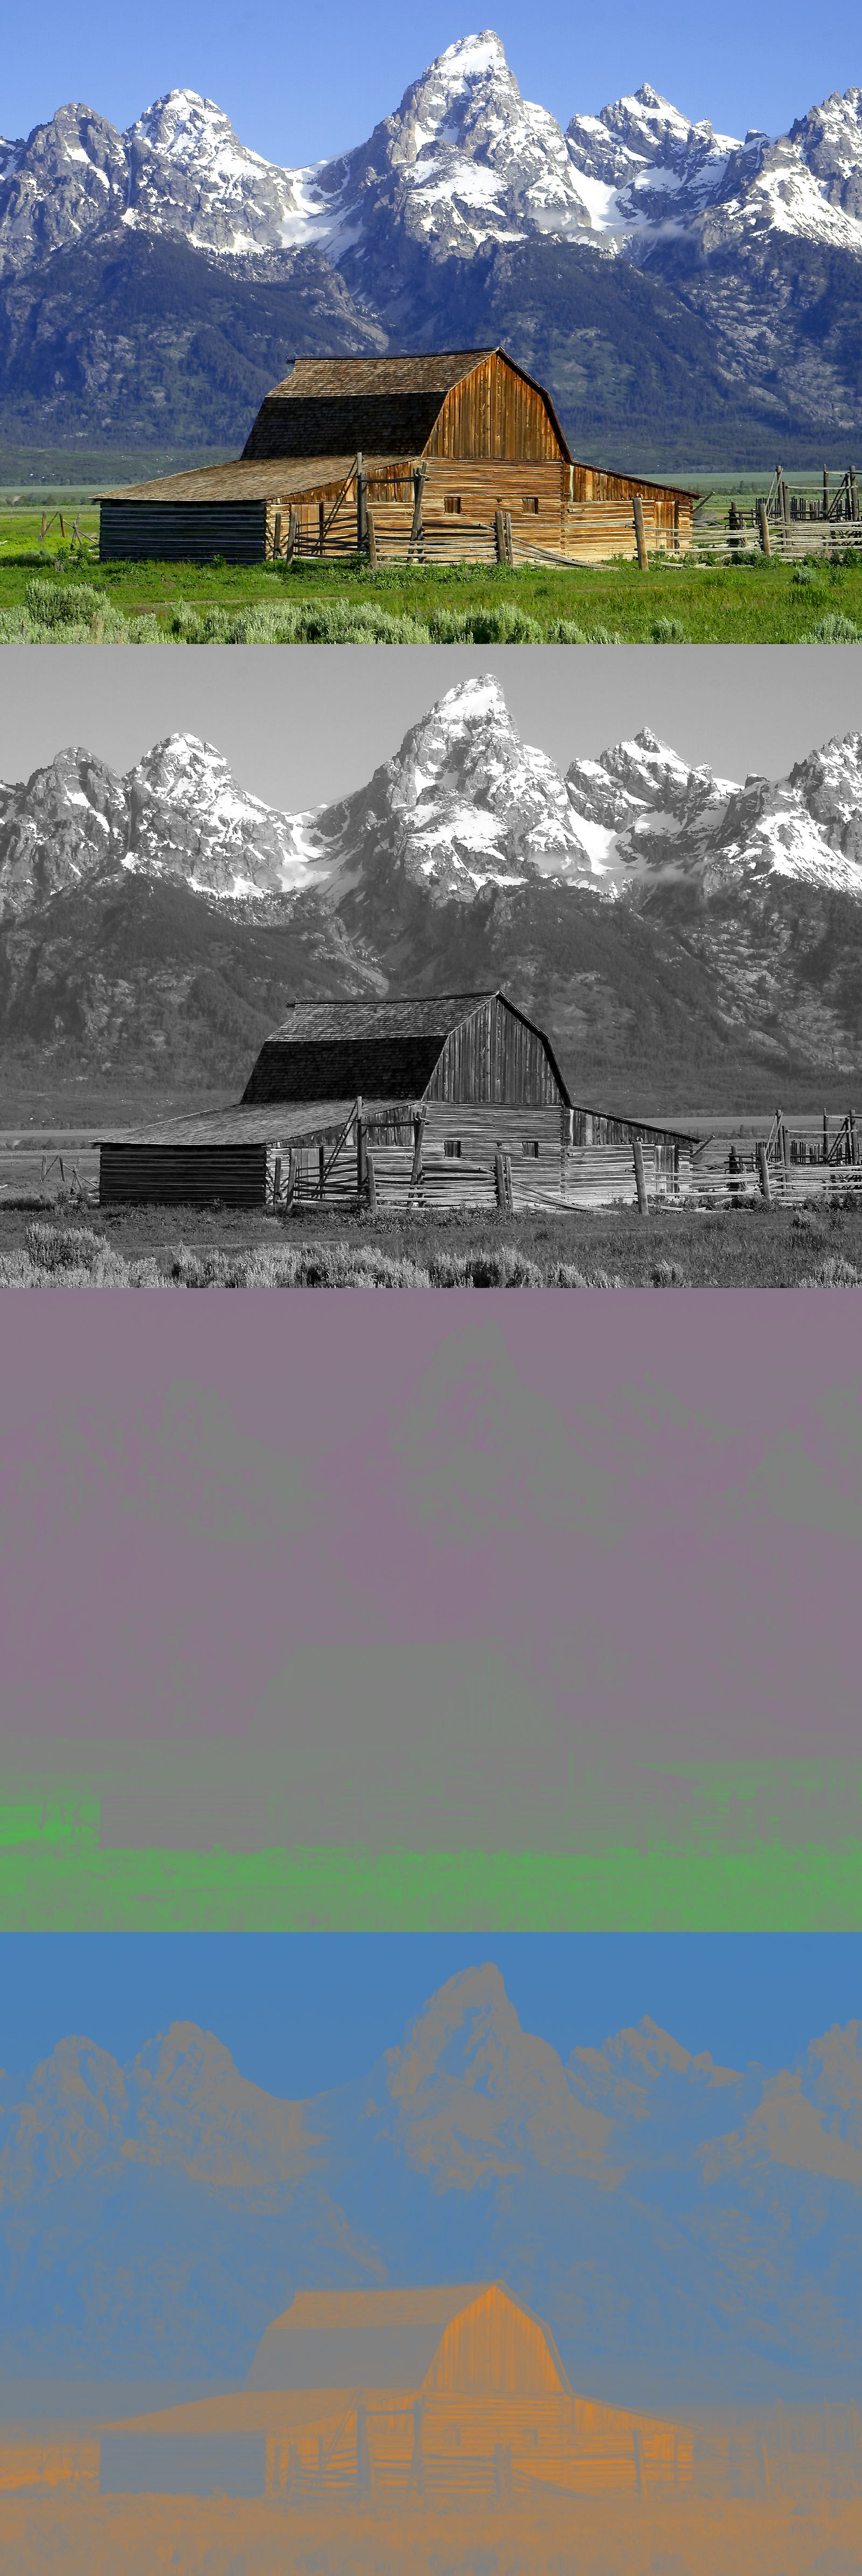
\includegraphics[height=10\baselineskip,keepaspectratio]{figures/Barns_grand_tetons_YCgCo_separation.jpg}
                \caption*{Source: \href{https://commons.wikimedia.org/wiki/File:Barns_grand_tetons_YCgCo_separation.jpg}{Devcore}, Public Domain, via Wikimedia Commons}
            \end{figure}
        \end{column}
    \end{columns}
\end{frame}

\begin{frame}{ICtCp}
    \begin{columns}<.->
        \begin{column}<.->{.7\textwidth}
            \begin{itemize}
                \item $(R, G, B)$ pixel $\rightarrow$ $(Y, Cb, Cr)$ signal values
                \item $Y$ is the \emph{luminance} signal
                      \begin{itemize}
                          \item Intuitively, our eyes are most sensitive to $G$
                          \item $G$ is a major contributor to the luminance value
                          \item $R$ and $B$ have smaller contributions
                      \end{itemize}
                \item $Cb$ and $Cr$ together form the \emph{chrominance} signal
                      \begin{itemize}
                          \item complementary \emph{colour difference} signals
                          \item $Cb$ blue - luma, $Cr$ red - luma
                      \end{itemize}
                \item Standardized by the ITU in two Recommendations
            \end{itemize}
        \end{column}
        \begin{column}<1->{.3\textwidth}
            \begin{figure}
                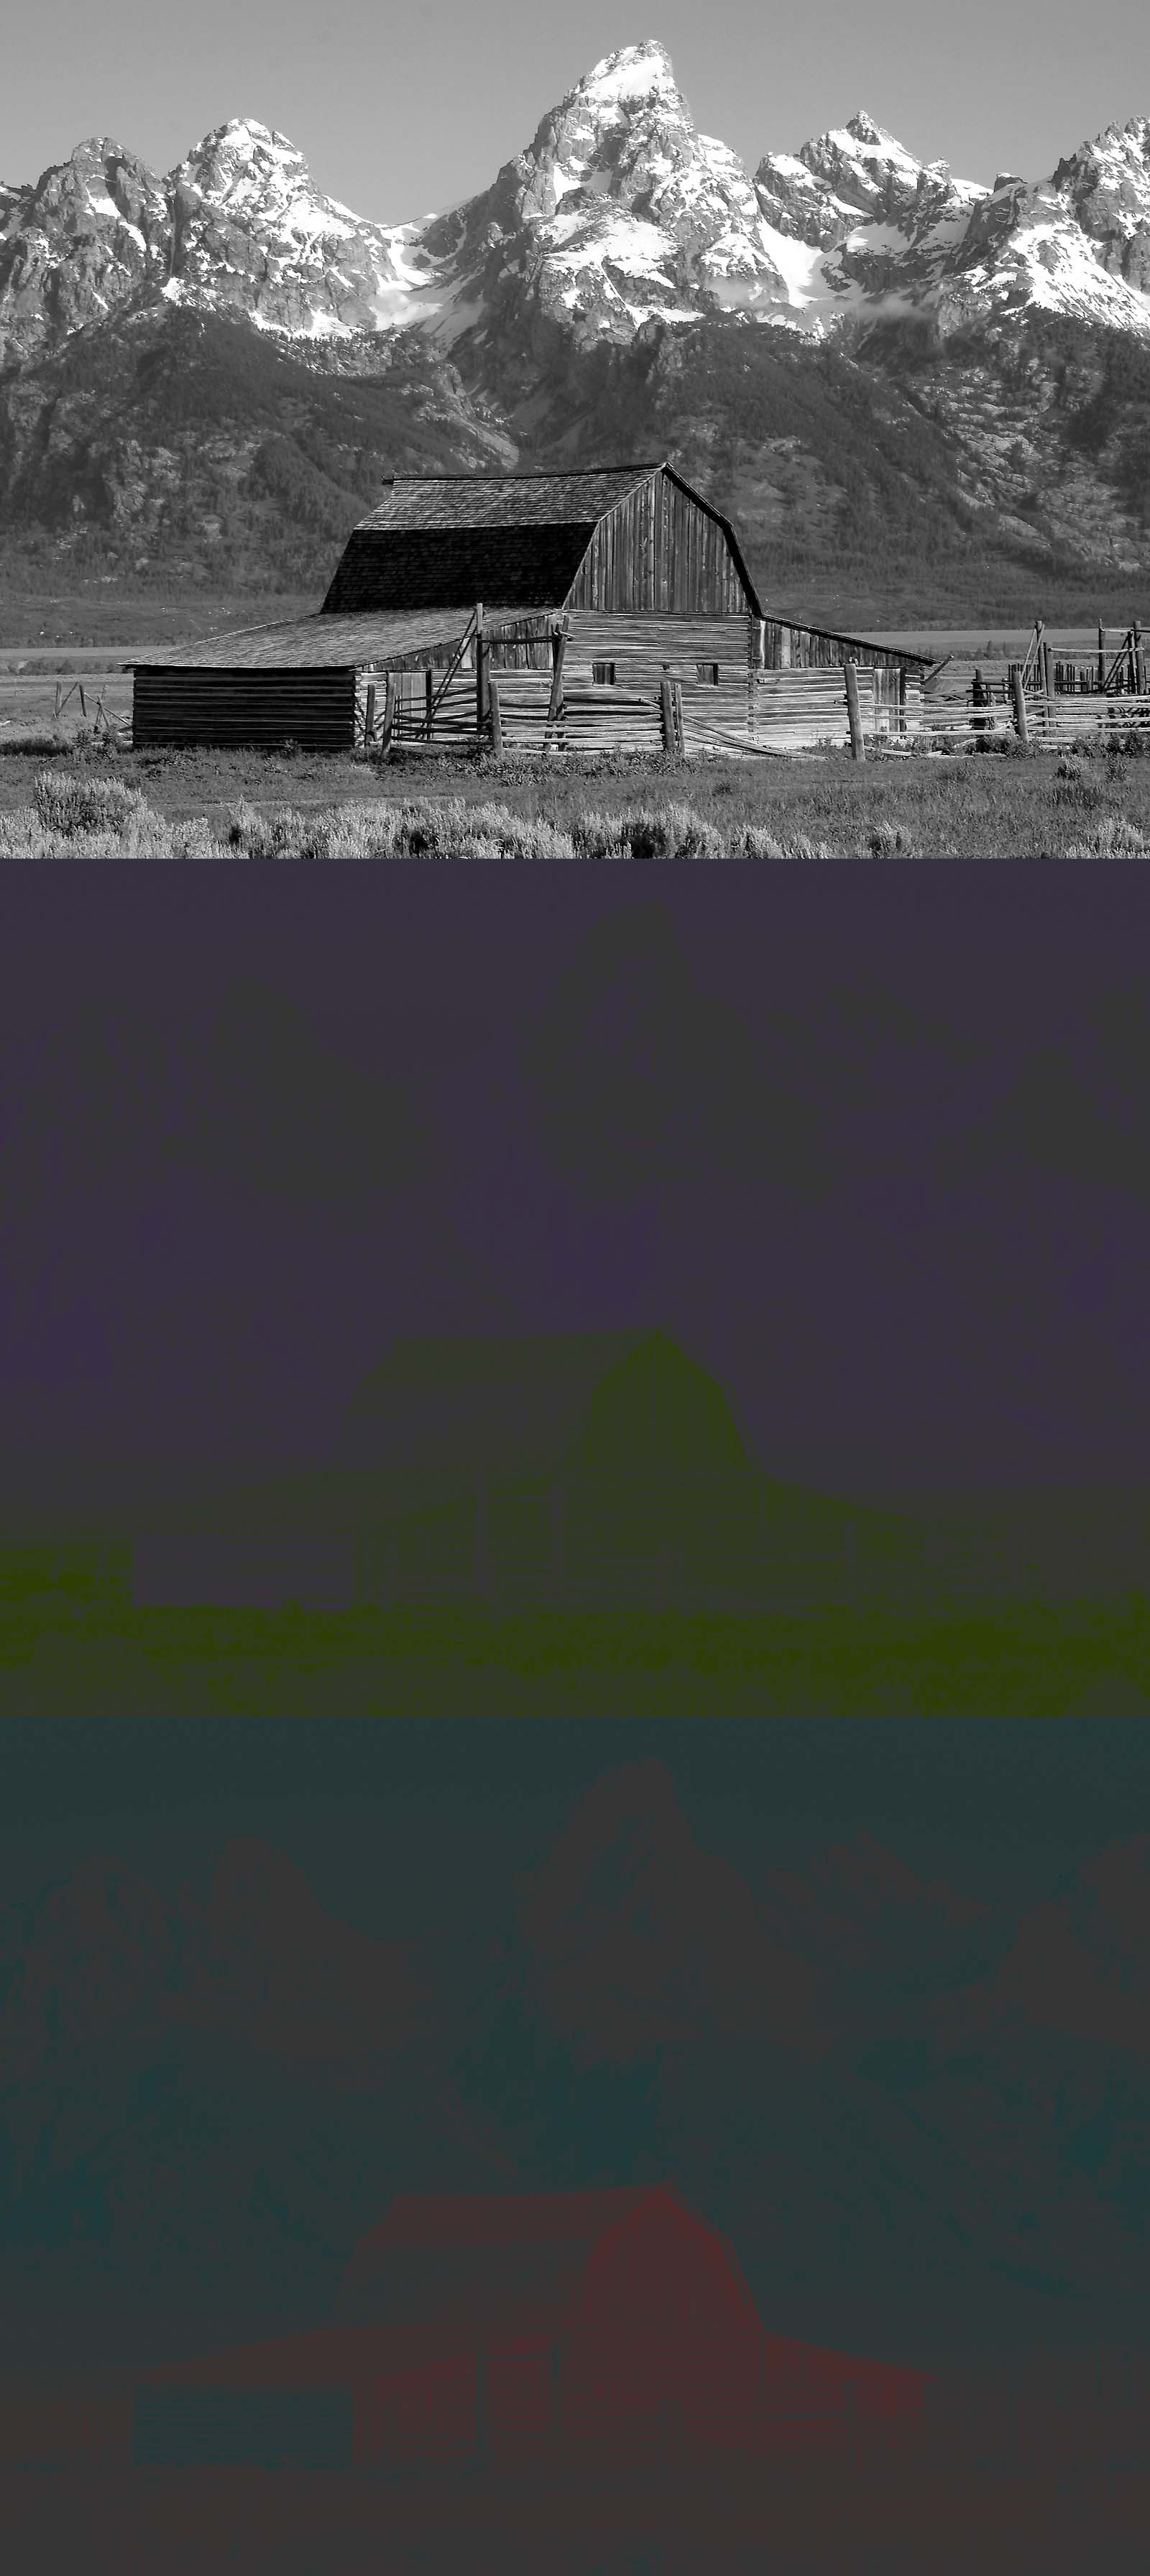
\includegraphics[height=10\baselineskip,keepaspectratio]{figures/ICtCp_components.jpg}
                \caption*{Source: based on \href{https://commons.wikimedia.org/wiki/File:Barns_grand_tetons.jpg}{Jon Sullivan (PD Photo.org)}, Public Domain, via Wikimedia Commons}
            \end{figure}
        \end{column}
    \end{columns}
\end{frame}
\section{Conclusions}
\begin{frame}{Remarks}
    \begin{itemize}
        \item Colour management is a complex beast
        \item A \emph{seriously} complex beast!
        \item We covered:
              \begin{itemize}
                  \item A primer on colour management
                  \item The uniqueness of the YCbCr colour space
                  \item How to turn a spec into a profile
              \end{itemize}
    \end{itemize}
\end{frame}
\begin{frame}{Remarks}
    \begin{itemize}
        \item We did not cover the actual implementation
        \item That would make for another hour of talk!
        \item The full, annotated profile generation code is available on GitHub
              \begin{itemize}
                  \item \faGithub~\href{https://github.com/amyspark/ycbcr-icc-profiles}{amyspark/ycbcr-icc-profiles}
              \end{itemize}
        \item Extra references at the end of this talk's slides
    \end{itemize}
\end{frame}
\begin{frame}{Thank you for watching!}
    \begin{center}
        {
            \large
            \textbf{Got any questions or comments?}
        }
        \begin{itemize}[<*>]
            \item Q+A next
            \item Email: \href{mailto:amy@amyspark.me?subject="FireShonks 2023"}{amy@amyspark.me}
            \item Matrix: \href{https://matrix.to/\#/@amyspark:fairydust.space}{@amyspark:fairydust.space}
        \end{itemize}
    \end{center}
\end{frame}
% https://tex.stackexchange.com/questions/30461/beamer-nonumber-equivalent-for-slides
\begin{frame}[plain,noframenumbering,allowframebreaks]{\bibname}
    \printbibliography[heading=none]
    \end{frame}
\end{document}
